% Author: Eskil Joergensen
% Tex Author: Magdalen Berns
% Formatting: Magdalen Berns

\chapter{Future Research in Retinal Imaging}

\label{future_research}
\lhead{\emph{Future Research in Retinal Imaging}}

The current technology for retinal imaging is rapidly developing.
With technological advances comes the potential for better
understanding of diseases associated with the retina, as well as
increased documentation of the biological structure of the retina.
Looking ahead this section will briefly introduce possible future
research areas, health concerns and uses of retinal imaging.

\section {Global Accessibility to Retinal Imaging}

Fundus cameras, \gls{cslo}s and \Gls{oct}s are
highly advanced retinal imaging machines which are commonplace in the
developed world. Their suitability for use in the developing world is
however somewhat superfluous, as a lack of trained photographers,
ophthalmologists and the inhibitive cost of these machines has prevented
wide-scale adoption. With over 90\% of visually impaired people living
in low and middle income countries the need to develop a suitable
retinal imaging device becomes clear.\cite{burgess2013diabetic}

The Ocular CellScope is a retinal imaging device which integrates the
camera of an iPhone with an indirect ophthalmoscope to capture
high-resolution images. With significant obstacles to retinal screening
in developing countries, the existence of affordable and portable devices that are
capable of retinal imaging are a great leap forward. With a total retail
cost of \pounds585 (compared with tens of thousands) the financial obstacle
to widespread clinical adoption is avoided. \Fref{fig:ocular} illustrates
the mechanical set-up of the Ocular CellScope, where the retina is
illuminated by an \Gls{led} flash that passes through the ophthalmic lens.
This device images in the same manner as the fundus camera which was
described in the previous section. The resulting retinal image has a 55$^\circ$ field of
view and a resolution of $2652\times2448$ pixels. \cite{medscape}

\begin{figure}[H]
\centering
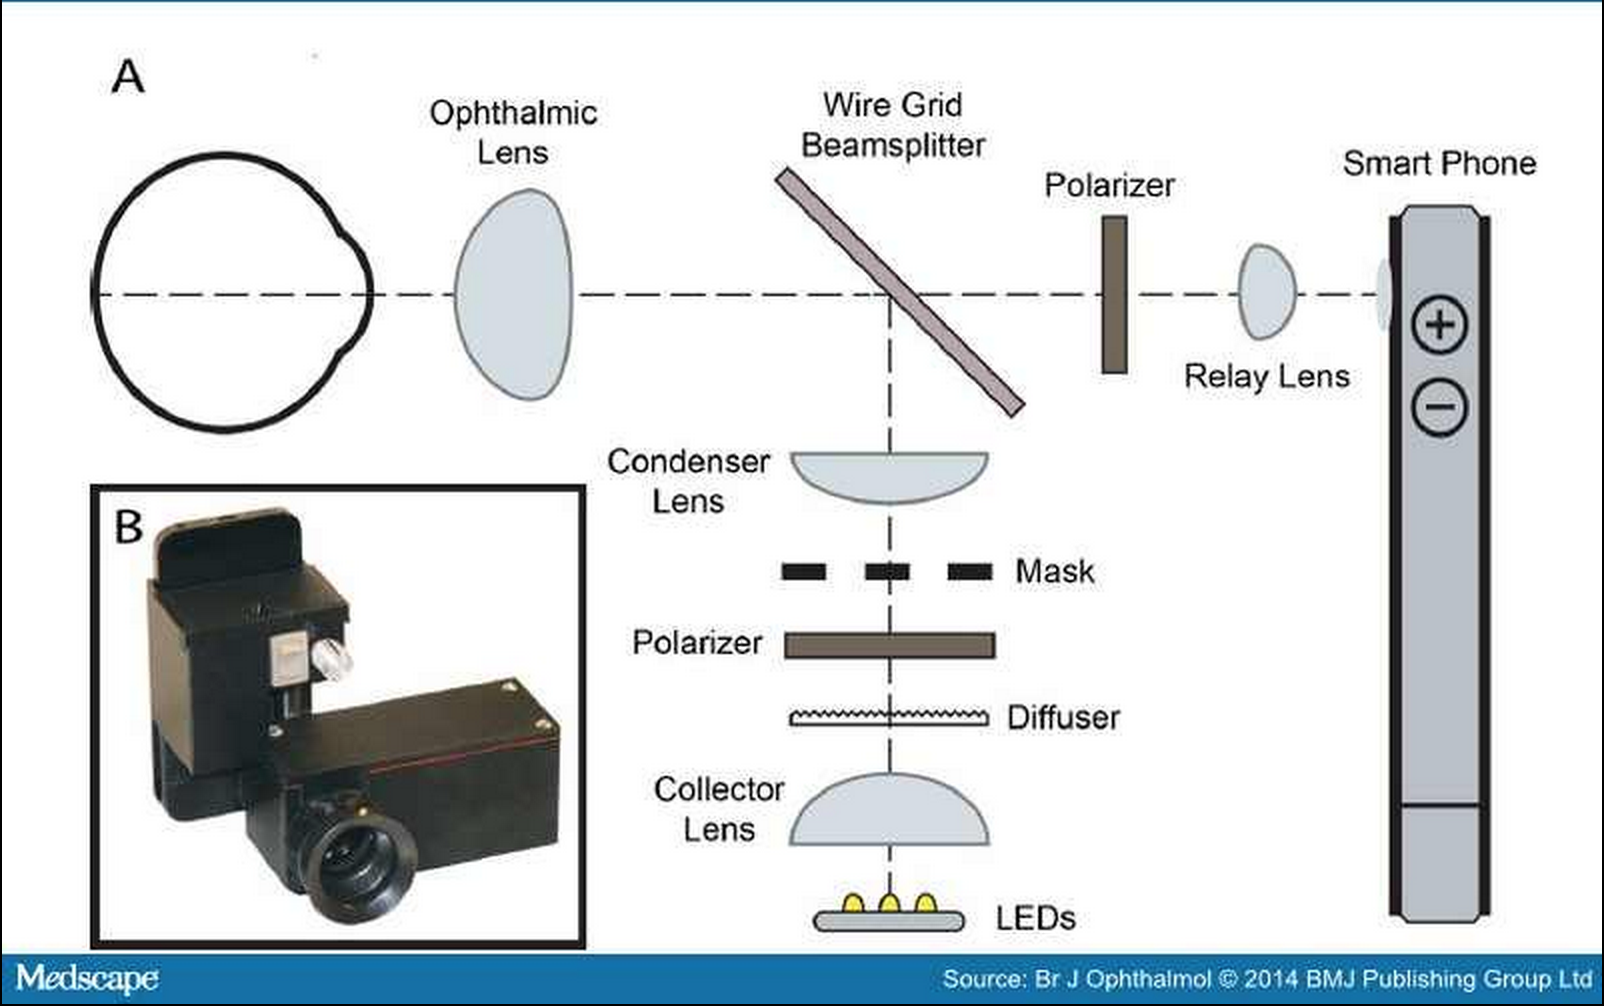
\includegraphics[width=12cm]{figures/ocular}
\caption{A schematic figure of the Ocular CellScope.\cite{medscape} }
\label{fig:ocular}
\end{figure}

The ocular cellscope serves a more general clinical need than the aforementioned
devices, where the goal is to diagnose the main causes of serious retinal pathology,
in order to reduce blindness in developing countries. As a result of dietary changes
the world faces the very real prospect of a diabetes epidemic, which is no longer
endemic to developed nations. \cite{burgess2013diabetic} The ability of the Ocular
CellScope to provide detailed images that aid in the diagnosis of diabetic retinopathy
is thus key to its viability. \Fref{fig:odr} shows the images obtained by the Ocular
CellScope, which clearly show the fatty fluid leakage and microaneurysms indicative of
diabetic retinopathy. By instituting national screening programmes along similar lines
to those adopted in the developed world, there would be a vast improvement in the early
diagnosis of retinal diseases, which in the case of diabetic retinopathy can reduce the
risk of blindness by 50\%. \cite{abramoff2010automated}

\begin{figure}[H]
\centering
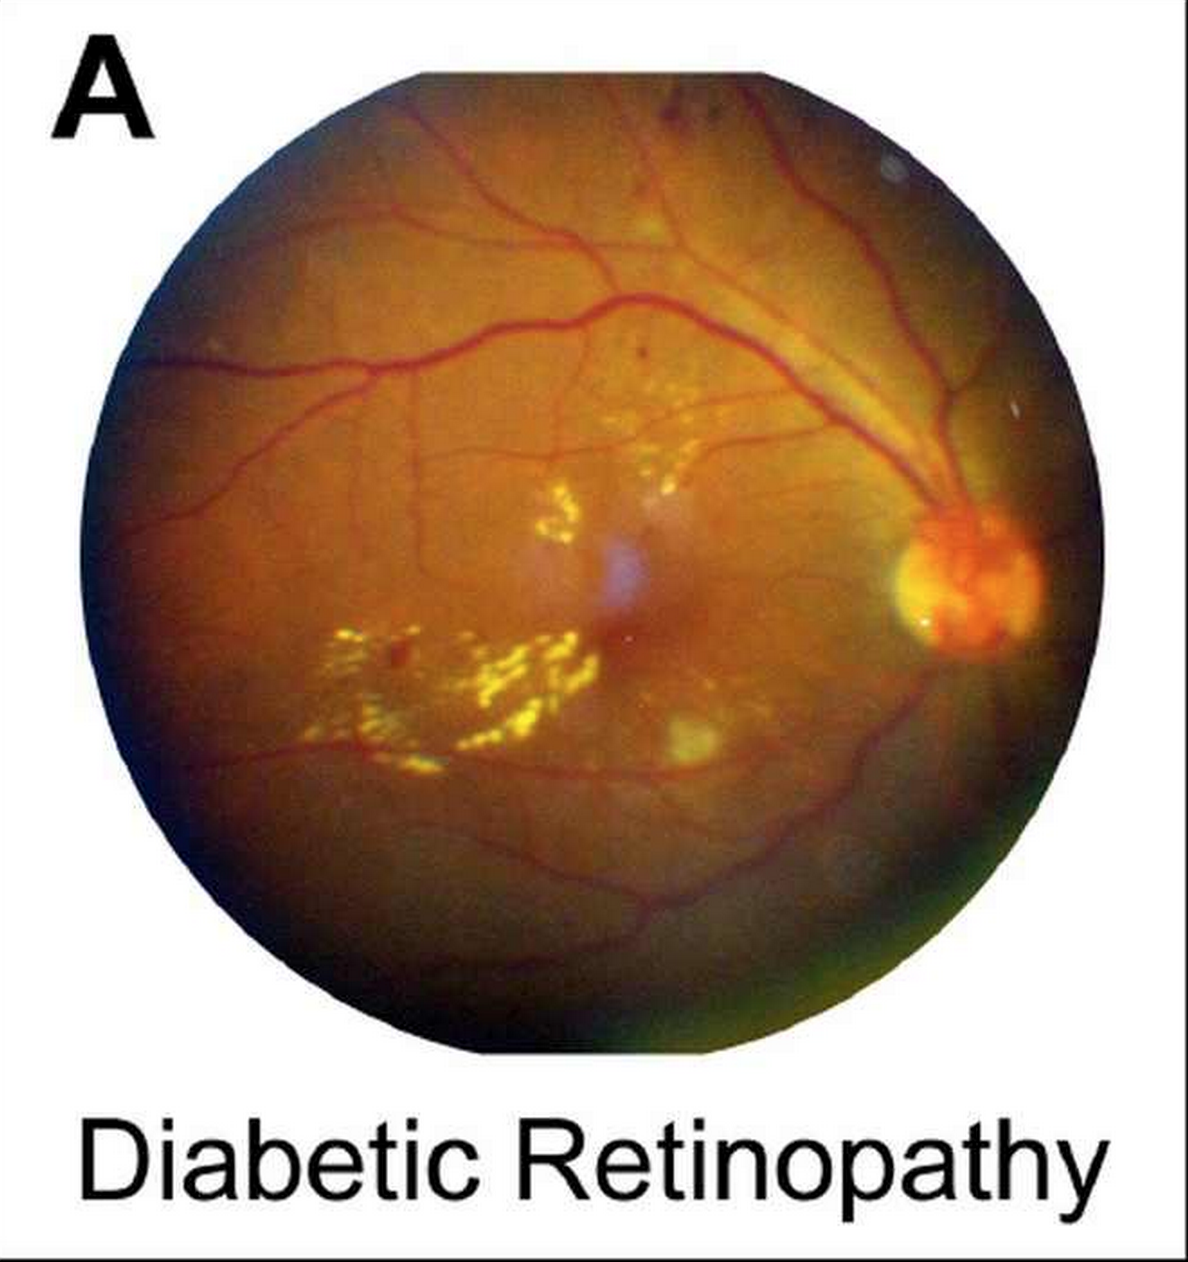
\includegraphics{figures/ocularDR}
\caption{A sample image of a patient with diabetic retinopathy using the Ocular
CellScope.\cite{medscape}}
\label{fig:odr}
\end{figure}

As was previously mentioned, the issues of the developing world are not just in simply
procuring equipment but also in the lack of trained people able to capture images and
perform image analysis. The connectivity and mobility of this device coupled with the
development of automated retinal screening programmes go a long way in solving these issues,
where images can be taken and then immediately sent to specialists for analysis. The
device has already been tested in Thailand, where the images were taken by untrained
personnel and then sent via mobile technology to a secure server, where ophthalmologists
have examined the images and returned a diagnosis. 

The development of automated early detection of diabetic retinopathy algorithms have
been a significant area of research in recent years. \Gls{cad}
is seen by many eye-care professionals as the most efficient way in reducing the
advancement of diabetic retinopathy and thus blindness in the developed and developing
world. In 2011 a study was conducted to test the ability of one \Gls{cad} system to detect
diabetic retinopathy on 1,200 images. The sensitivity of the algorithm was compared
against the sensitivity of two specialist graders and was comparable in accuracy.
\cite{sanchez2011evaluation} \Fref{fig:autodr} is an example of a successful detection
by the software, which would then be referred to a specialist for consideration.

\begin{figure}[H]
\centering
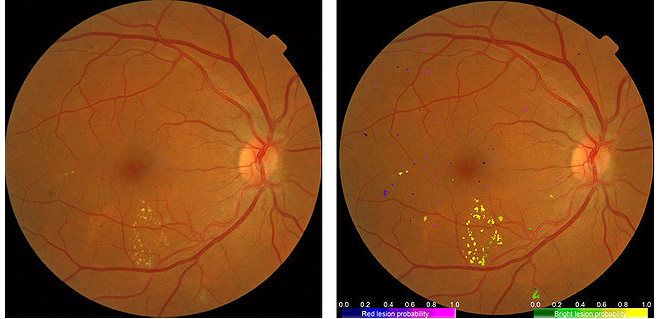
\includegraphics{figures/autodr}
\caption{An image illustrating the ability of the algorithm to detect fatty fluid leaks
and haemorrhages in a patient suffering from diabetic retinopathy. The image on the left
is the standard colour fundus. The image on the right demonstrates the detection of
symptoms by the software.\cite{sanchez2011evaluation}}
\label{fig:autodr}
\end{figure}

By combining portable and affordable retinal imaging devices with an accurate automated
detection system, the possibility of having effective retinal screening programmes in the
developing world is very real and imminent.


\section{Blue light hazard}

The prevalence of blue-light \Gls{led} in modern technology has led many to consider
the possible detrimental effects of over-exposure on the retinal tissue. The
fast-growing use of \Gls{led} devices and energy-efficient light bulbs, with a peak
light-wavelength in the blue light region, can cause significantly increased oxidative
stress on the retinal tissue.\cite{shang_wang} A chronic exposure to blue light can
result in induced photochemical deterioration of the retina, which has the effect of
accelerating the biological ageing process.\cite{behar_cohen_2011}

\begin{figure}[H]
\centering
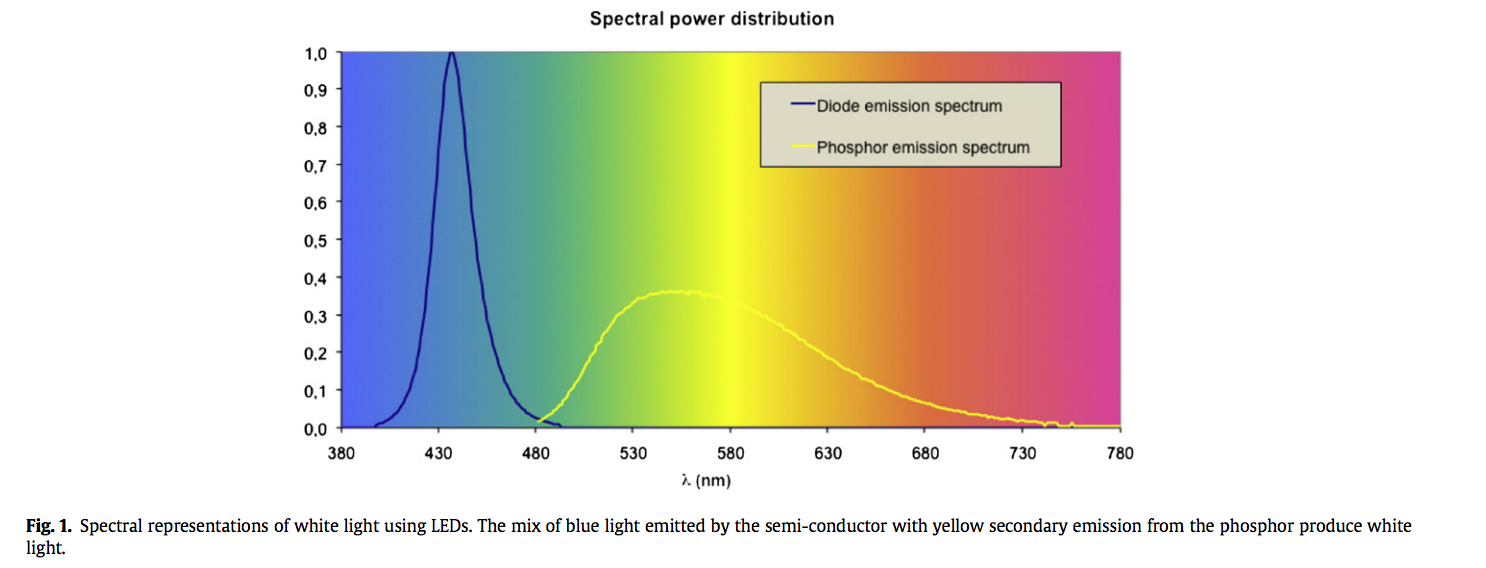
\includegraphics[width=12cm]{figures/bluehazard}
\caption{A sample image of a patient with diabetic retinopathy using the Ocular CellScope.\cite{behar_cohen_2011}}
\label{fig:bluehaz}
\end{figure}


Normal white light, as well as sunlight, contains a wide distribution of all colour
wavelengths. \Fref{fig:bluehaz} shows how the wavelengths of a white-light \Gls{led} and a
traditional light bulb are distributed. Light of different wavelength are either absorbed
or transmitted by different sections of the eye. As a result, being exposed to natural
sunlight means that the different sections of the eye are all used. By introducing a
narrow range of light waves means that some parts of the eye will be used more than
others. In the case of blue-intensive light waves, those are all absorbed by
the retina alone, as can be seen in \fref{fig:wl}.

\begin{figure}[H]
\centering
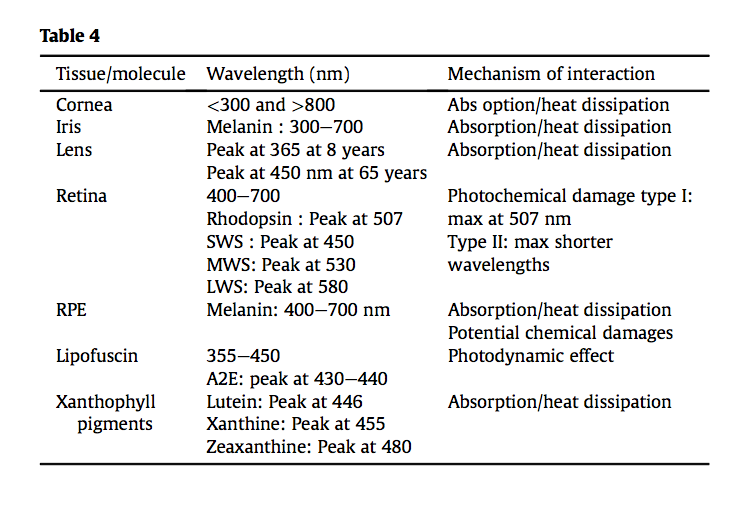
\includegraphics{figures/wavelength}
\caption{A table showing how light of different wavelengths are handled inside the eye.\cite{behar_cohen_2011}}
\label{fig:wl}
\end{figure}

As everyday use of blue-intensive light sources is relatively new, the long-term
effects are yet to be fully understood. In a study on the effect of blue light on the
ocular health of rhesus monkeys, it was observed that high intensity exposure
for 1,000 seconds resulted in the inflammation and subsequent damage of the
retinal pigment epithelial. \cite{ham1980nature} These findings are not yet
validated for humans, but with the prevalence of blue light in modern technology
the effects will become more observable in time. Hence the development of retinal
imaging techniques are important in gathering information about the biological
effects of blue-light and maintaining the study of these trends.

\section{Multimodality}

Multimodality imaging is the simultaneous capturing of retinal images in the various
aforementioned modalities, and blending the various fundus modes with an \Gls{oct}
image.\cite{abramoff2010retinal} This allows for direct comparison of pathology
across the various modes and thus presents the ultimate diagnostic tool for
ophthalmologists. For image information from multiple modalities to be usable in a
mutual context, images must be registered independently. This is achieved in
practice by individually capturing each image over a very short period of time
and then concatenating these descriptions to form one multimodal image, as
shown in \fref{fig:mt}.

\begin{figure}[H]
\centering
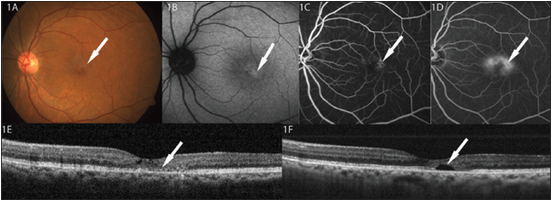
\includegraphics{figures/multitwo}
\caption{Multimodal image of a patient with macular leakage. 1A is a colour fundus
photograph, where the arrow indicates the greying of the tissue. 1B is a fundus
autofluorescence image with a small increase in macular autofluorescence. 1C and 1D
are fluorescein angiograms at early and late stage respectively, these images illustrate
the leaking from the vessels. 1E and 1F are spectral domain \Gls{oct} images which
demonstrate foveal thinning and retinal damage.\cite{abramoff2010retinal}}
\label{fig:mt}
\end{figure}

\Fref{fig:mt} illustrates the diversity multimodal imaging brings and how each mode
can provide the clinician with a different piece of information to aid successful
diagnosis. Additional retinal imaging techniques such as hyperspectral imaging,
oximetry, and adaptive optics \gls{cslo}s are being developed and will contribute more
clinical information once they are fine tuned.

Optos have developed a multimodality option which spatially maps the 3-D \Gls{oct}
image on top of the 2-D retinal scan image. This feature illustrates the structural
defects beneath the image and is used to show how symptoms manifest differently in
each modality, an example of this is shown in \fref{fig:multi}.

\begin{figure}[H]
\centering
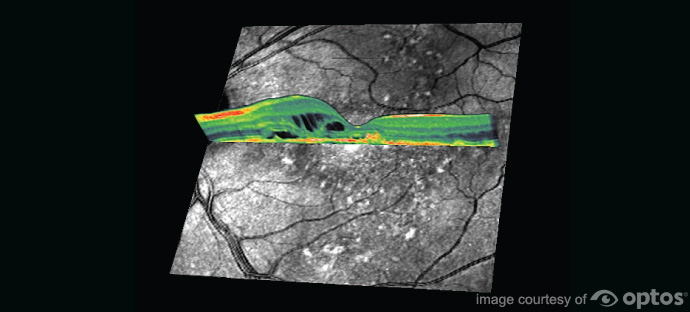
\includegraphics{figures/multi}
\caption{Combination of \Gls{cslo} retinal image and \Gls{oct} image in a patient
suffering from dry \Gls{amd}. The images both illustrate the accumulation of
drusen in Bruch's membrane (the innermost layer of the choroid).\cite{optos_2015}}
\label{fig:multi}
\end{figure}

\section{Adaptive Optics and High Resolution Imaging}


As was mentioned earlier, one of the physical limitations in retinal imaging is
the optical resolution as a result of diffraction. This limitation affects both
typical systems, such as the Topcon TRC-NW8F, and more advanced systems, such as
the Optos California and the \Gls{oct}. This fundamental resolution limit couples with
the blurring caused by aberration in the optical system to give maximum optical
resolutions around 20 microns for devices at normal operating distance from the
eye (10-40mm). Recent studies \cite{barber2003new} have suggested that diseases
initially thought to be contained to the vascular network, for instance diabetic
retinopathy, actually manifest themselves in the cellular makeup of the eye. The
current instruments are unable to image cells individually as the foveal cones
have a diameter between 3-5 microns; hence diagnosis of disease based on cellular
pathology is impossible. The diffraction limit of resolution for an imaging system
at 10mm from the eye is between 2-5 microns, dependent on the visual acuity of the
patient. Hence high-resolution images of ocular cells are practically obtainable
if aberration is reduced to zero.
 
\Gls{ao} is a method of removing all aberration from an optical system
through the use of a deformable mirror, which transforms and reverses the wavefront
distortions caused by system imperfections. This technology, which was originally
developed for use in telescopes, has recently been applied to retinal imaging
devices with great success. \cite{zhang2006high} With this new capability
practitioners are able to successfully image the retinal cones, opening up a vast
new area of research in pathology at a cellular level. \Fref{fig:ao} illustrates
\Gls{ao} with a fundus camera.

\begin{figure}[H]
\centering
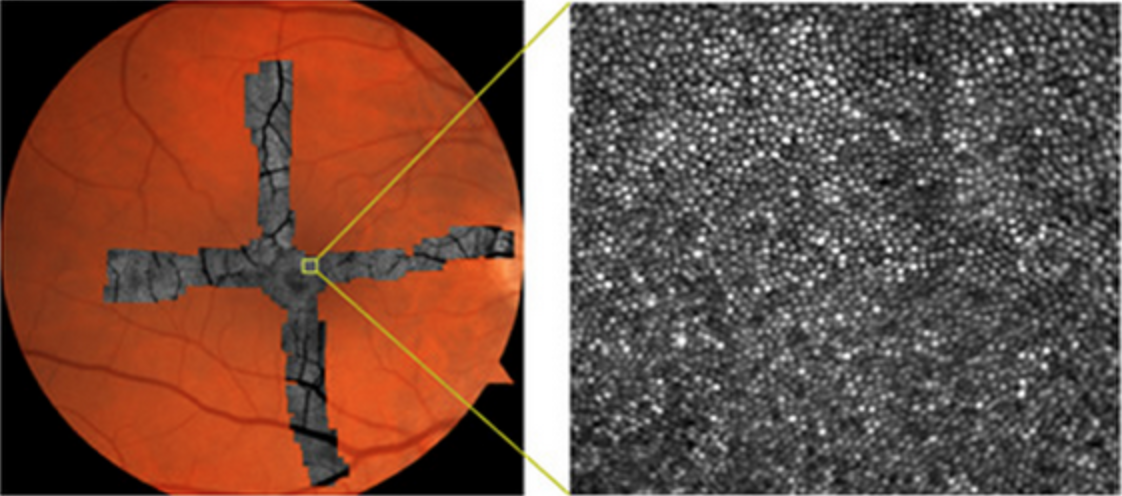
\includegraphics{figures/ao}
\caption{A comparison of standard resolution fundus images with the
              capability for high resolution \Gls{ao} imaging.\cite{zhang2006high}}
\label{fig:ao}
\end{figure}

\section{Two-Photon Retinal Microscopy}

Having introduced the issue of retinal damage as a result of blue-light
absorption and the blue-light reliant imaging technique of \Gls{faf}, the reader may have deduced a conundrum facing ophthalmologists. Currently
practitioners face the issue of causing harm to the patient in order to retrieve
valuable diagnostic information from \Gls{faf} imaging. A novel method has been proposed
to avoid this problem altogether; two-photon retinal microscopy.

Recently it has been shown that fluorescent retinal tissue exhibits a non-linear
response to incident radiation. \cite{denk1990two} There exists a probability of
two-photon absorption by the organic material which is proportional to the square
of the intensity of the light beam. With this method a normally blue absorbing
tissue will instead reach its excited state by absorbing two photons of double
blue wavelength(near IR). This means that harmless radiation wavelengths can be used to
observe fluorescent properties of tissue, if the correct powers of beam are
achieved. By using a high intensity (50mW) and short pulse (100fs) \Gls{laser}
beam the desired properties of the incident radiation can be achieved without causing
harm to the retina. Further development in this field is expected, with recent studies
linking information obtained through this method with symptoms of \Gls{amd}
and other retinal defects.\cite{palczewska2010noninvasive,palczewska2014noninvasive}

\section{Security}

The unique retinal vascular pattern has many applications, most notably in
personal security and protection. A security system can be designed to recognise
the unique biometrics of the eye (iris and retina) and grant access based on
matching information. The pattern of the retina, which maps the locations
of veins, arteries, the macula and the optic nerve in the eye, has a much
more complex pattern than the normally used fingerprint or iris.\cite{ortega_2009}

The retinal images are then analysed using complex computer algorithms,
converted to computer code and then saved in a database. Presently one
of the most commonly used algorithms for both saving and matching retinas
is a version of the \Gls{sift}. \Fref{fig:sift} shows an image of the process,
where the \Gls{sift} algorithm is trying to match keypoints from from retinas.
Simply put the \Gls{sift} algorithm takes key features from the image and
saves a vector collection in a database. In the matching process an object is
recognised by comparing the new vector set with the ones in the database.
The matching is often computed very efficiently using a best-bin-first search
algorithm, that begins with a keypoint and moves outward from that.

\begin{figure}[H]
\centering
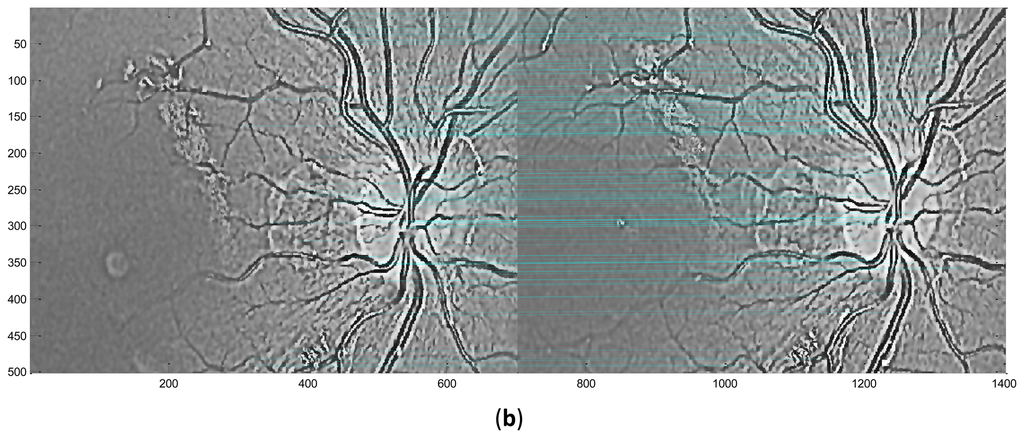
\includegraphics{figures/sift}
\caption{An example of the \Gls{sift} used to produce a retinal fingerprint
              to match retinal scans to the database.\cite{Martinez-Perez:12}}
\label{fig:sift}
\end{figure}

The retina contains at least as much individual data as a fingerprint. 
However, unlike a fingerprint, it is an internal organ and is less susceptible
to either intentional or unintentional modification. Where a thumb can be
amputated and still be used in a scanner, the blood vessels mapping across
the retina would contract quickly, so that having someone's removed eye
would not help in tricking a retinal recognition scanner. Normally the retina's
intricate network of blood vessels is a physiological characteristic that
remains stable throughout the life of a person. However, certain eye-related
medical conditions and diseases, such as cataracts and glaucoma, can render
a person unable to use retina-scan technology, as the blood vessels can
be obscured.\cite{rarr_2015}  In terms of consistency a retina scan has an
error rate of 1 in 10,000,000, whereas the error of a fingerprint scan can be as
high as 1 in 500.

